\chapter{Recorrido de Campo}

El recorrido de campo se realiz\'o entre los d\'ias 22 y 24 de Noviembre de 2017. La zona recorrida se tuvo como prop\'osito inspeccionar aquellos lugares que mostraron menor factor de seguridad en las pruebas preliminares y apreciar el estado de las unidades geol\'ogicas que muestra la cartograf\'ia estudiada. 

En campo se pudo corroborar la consistencia de la unidad geol\'ogica predominante Ksaau (limolita), dicho material se pudo apreciar en todo el recorrido, con leve variaci\'on en su grado de meteorizaci\'on, principalmente en zonas de abundante vegetaci\'on. La morfolog\'ia abrupta de las laderas permiti\'o apreciar abundantes cicatrices de anteriores desprendimientos de material, principalmente en sectores de alta pendiente y en el trazado de la carretera el Carmen- choc\'o.

Se realizaron 2 estaciones en las cuales se realiz\'o la respectiva toma de muestra, siendo la primera de ellas la que m\'a s informaci\'on proveer\'ia en los posteriores ensayos de laboratorio. Para la toma de muestra se tuvo la precauci\'on de seleccionar un lugar que no presentase retrabajamiento del material y en el cual se pudiese observar que el suelo presentase unas condiciones representativas del material observado durante los recorridos realizados.
Las muestras tomadas en la segunda estaci\'on se tomaron a una profundidad m\'a s somera con la intenci\'on de, posteriormente, poder obtener los par\'a metros de resistencia de instancias m\'a s avanzadas de meteorizaci\'on de la limonita. Esto dado que las cicatrices de movimientos en masa observadas aparentaban que aquellos eventos ocurridos se dieron hace un tiempo considerable(a juzgar por el crecimiento nueva cobertura vegetal) no contaron con profundidades considerables de su respectiva superficie de falla. Asimismo, testimonio obtenido de una habitante del lugar, corrobora que no son frecuentes movimientos que comprendan altos vol\'umenes de material, habiendo ocurrido el \'ultimo aproximadamente 5 a�os antes de la visita de campo.

La estaci�n 1 se realiz� en las coordenadas \textbf{5.8712778,-76.0848778}, mientras que la estaci�n 2 se realiz� en las las coordenadas \textbf{5.8612472,-76.0927833} :

\textbf{Muestras recolectadas}



De la estaci�n 1 se obtuvo:
\begin{itemize}
  \item Muestra al interior de 4 tubos PVC de 2 pulgadas de di�metro y aproximadamente 15 cm de alto.
  \item 1 Bloque de muestra inalterada  de aproximadamente 40cm x 40cm x 30cm.
  \item 200gr de muestra alterada..
\end{itemize}

De la estaci�n 2 se obtuvo:
\begin{itemize}
  \item Muestra al interior de 3 tubos PVC de 2 pulgadas de di�metro y aproximadamente 15 cm de alto.
\end{itemize}

 

 


\begin{figure}[H]
\centering
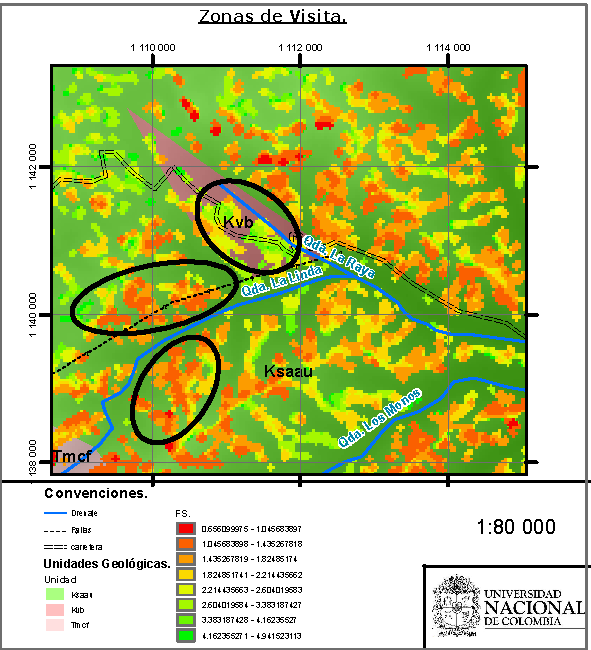
\includegraphics[scale=1]{img/visita.pdf}
\caption{Zonas de visita propuestas, se marcaron las zonas con mayor y menor resultado de Factor de Seguridad.}
\label{fig:campo}
\end{figure}

\section{Conclusiones}


\section{Recomendaciones}

